\documentclass[pdftex,12pt,a4paper]{article} 
% margin size
\usepackage[margin=1in]{geometry}
% t1 encoding so underscores in \texttt render and copy as real characters
\usepackage[T1]{fontenc}
\usepackage{lmodern}

% Math and algorithms
\usepackage{amsmath,amssymb,amsthm,esint}  % For both in-line and equation mode
\usepackage{bbm}
\usepackage{mathdots}
\usepackage{bm}
\usepackage{algorithm}
\usepackage{algorithmic} % Algorithm styles, need to be nested for the example shown
\usepackage{aliascnt}
\numberwithin{equation}{section} % Numbering of our equations per section
\newtheorem{theorem}{Theorem}
\newtheorem{definition}{Definition}
\newtheorem{proposition}{Proposition}
\newtheorem{corollary}{Corollary}
\newtheorem{remark}{Remark}

\usepackage{setspace} %Spacing on the front page for crest and titles
\usepackage[]{fncychap} % Styles can be Sonny, Lenny, Glenn, Conny, Rejne, Bjarne and Bjornstrup
\usepackage[hyphens]{url} % Deals with hyphens in urls to make them clickable
\usepackage{xcolor} % Great if you want coloured text

% Figures
\usepackage{wrapfig}
\usepackage{graphicx} % Inserting images
\graphicspath{ {figures/} } 
\usepackage{caption}
\usepackage{float}

% Tables
\usepackage{tabularx}
\usepackage{multirow} 
\renewcommand{\arraystretch}{1.15}
\usepackage{booktabs}
% notebook-generated table bodies; the primitive input is expandable, so \bottomrule may follow it
\makeatletter\newcommand{\tablebody}[1]{\@@input tables/#1.tex }\makeatother

% Appendix
\usepackage{appendix} 

\usepackage{natbib}
\usepackage{comment}

% Tikz figures
\usepackage{tikz}
\newcommand{\ImageWidth}{14cm} 
\usetikzlibrary{decorations.pathreplacing,positioning, arrows.meta} 

% Fancy headers and footnotes
\usepackage{fancyhdr}
\usepackage[symbol]{footmisc}
\renewcommand{\thefootnote}{\fnsymbol{footnote}} 

% Hyperlinks and auto-references
\usepackage[hidelinks]{hyperref}  
\def\sectionautorefname{Section}
\def\appendixname{Appendix}
\newcommand{\propositionautorefname}{Proposition}
\newcommand{\definitionautorefname}{Definition}
\newcommand{\corollaryautorefname}{Corollary}  

\setlength{\footnotesep}{0.5cm}
%%%%%%%%%%%%%%%%%%%%%%%%%% DOCUMENT STARTS %%%%%%%%%%%%%%%%%%%%%%%%%%%%% 

\begin{document} 
% Front page 
\pagestyle{empty}

% Logo, Title
\begin{center}
	\begin{figure}
		\centering
		
\includegraphics[scale=0.8]{tec_logo.png}
		\vspace{10mm}
	\end{figure}
	\textbf{\begin{huge}
		Algorithmic Analysis of\\ Water Distribution Networks \\
	\end{huge}}
	\vspace{10mm}
\end{center}

% Subject, Code and Date
\begin{center}
	\vspace{5mm}
	\textbf{\large Analysis and Design of Advanced Algorithms (Gpo 605)}\\
    {\large TC2038, Situation Problem 2\\}
	\vspace{5mm}
	\textbf{\large Santiago Hernández Senosiain\\}
	\large A01787550 \\
\end{center}

\begin{center}
    \vspace{10mm}
	November 2, 2026 \\
	\vspace{2mm}
\end{center}
  
%\renewcommand{\headrulewidth}{0pt} 
\tableofcontents
\clearpage
\renewcommand{\thefootnote}{\arabic{footnote}}
\pagestyle{fancy}
\fancyhf{}
\setlength{\headheight}{14.49998pt}
\addtolength{\topmargin}{-2.49998pt} 
\lhead{Algorithmic Analysis of Water Distribution Networks}
\def\layersep{2.5cm}
\pagenumbering{arabic}
\lfoot{\centering \thepage}
\onehalfspacing 

% Sections
\section{Problem definition}\label{sec:problem}
A water distribution network is an undirected graph $G=(V,E)$ whose vertices are junctions with coordinates $p_v\in\mathbb{R}^2$, a subset $S\subseteq V$ of which are sources, and whose edges are pipes with a capacity $c(u,v)>0$. The length of a pipe is $\ell(u,v)=\lVert p_u-p_v\rVert_2$ and $d_G(u,v)$ denotes the shortest-path distance under $\ell$. The Water Graph Problem \citep{narvaez_slides} poses seven questions on this model, and the situation problem brief \citep{tc2038_brief} asks each student to investigate one of them. With the instructor's approval, this report covers all seven as a single study, because their results feed each other: lengths define distances, distances define sectors, sectors define the flow problems.
\begin{enumerate}
    \item[\textbf{T1}] \textbf{Representation.} Build adjacency-list and adjacency-matrix representations, explore $G$ with BFS and DFS, find its connected components, and compare time and memory of both representations.
    \item[\textbf{T2}] \textbf{Pipe lengths.} Compute $\ell(u,v)$ for every pipe, the shortest, longest and total length, and compare straight-line distance $\lVert p_u-p_v\rVert$ with network distance $d_G(u,v)$.
    \item[\textbf{T3}] \textbf{Sectorization.} Assign every node to $\sigma(v)=\arg\min_{s\in S}d_G(s,v)$ and find the pipes to close: $C=\{(u,v)\in E:\sigma(u)\neq\sigma(v)\}$.
    \item[\textbf{T4}] \textbf{Freshness.} Water age is proportional to $d_G$. For each sector $V_s=\sigma^{-1}(s)$ find the farthest node $t_s=\arg\max_{v\in V_s}d_G(s,v)$, its distance and its route.
    \item[\textbf{T5}] \textbf{Maximum flow.} In each sector, maximise the flow from $s$ to $t_s$ subject to $|f(u,v)|\le c(u,v)$ and flow conservation, and identify the bottleneck pipes.
    \item[\textbf{T6}] \textbf{Sampling route.} Find a minimum-length closed walk that starts and ends at the node labelled office and visits every node. Nodes and pipes may be repeated, since $G$ need not contain a Hamiltonian cycle.
    \item[\textbf{T7}] \textbf{Expansion.} Link a new point $q$ by one pipe to its nearest non-source node, $\arg\min_{v\in V\setminus S}\lVert p_v-q\rVert$, and update both representations.
\end{enumerate}

\section{Datasets}\label{sec:datasets}
The four instances provided with the challenge (NYT, HAN, FOS, PES) are text files with a \texttt{V E} header and four sections: \texttt{[NODES]} (\texttt{id x y source\_flag}), \texttt{[EDGES]} (\texttt{u v capacity}), \texttt{[OFFICE]} (office id, T6) and \texttt{[NEW]} (\texttt{x y capacity} of nodes to insert, T7). Node attributes are id, coordinates and source flag; the only edge attribute is the third column, which the slides call the pipe capacity and label as the diameter in their figures \citep{narvaez_slides}. It is used as capacity in T5 and never as length. Table~\ref{tab:datasets} summarises the instances.

\begin{table}[H]
\centering\small
\caption{Instances after validation. Loops: independent cycles $E-V+1$; Caps.: distinct capacity values.}\label{tab:datasets}
\begin{tabular}{lrrrrrrrrrr}
\toprule
\tablebody{datasets}
\bottomrule
\end{tabular}
\end{table}

\paragraph{Validation.} The loader logs, instead of failing on, malformed or non-finite values, pipes to unknown nodes, self-loops, non-positive capacities, repeated pipes, coincident coordinates, id gaps, header mismatches, a missing office, and \texttt{[NEW]} points outside the network's bounding box enlarged by 50\%. No value is missing or invalid, but three things are unexpected. PES lists pipe 28--30 twice (as \texttt{28 30} and \texttt{30 28}, same capacity); it is kept once, so PES has 98 pipes, not the declared 99, and that pipe's capacity is not doubled in T5. PES ids have 18 gaps, handled by an id-to-index map. NYT's second \texttt{[NEW]} point $(6478,3050)$ lies about five network widths east of NYT and equals HAN's second entry, so it is treated as a copy error and not inserted.

\paragraph{Structure.} All instances are connected and have two sources. NYT and HAN are almost trees, FOS and PES are meshed. Six of the eight sources are leaves (both in NYT and HAN, 37 in FOS, 7 in PES), joined to the network by a single pipe. All four networks are very sparse, with density $2E/(V(V-1))$ between 0.039 (PES) and 0.111 (NYT).

\section{Algorithm}\label{sec:algorithm}
Each task is matched to a TC2038 technique that fits its structure, and each main algorithm is compared with an alternative or a baseline.

\subsection{T1: graph traversal}
Connectivity is a reachability question that involves no weights, so graph traversal is sufficient. BFS (with a FIFO queue) and DFS (with an explicit stack) each visit every vertex reachable from the start exactly once; restarting from each vertex not yet visited yields the connected components. Both traversals run on the adjacency list, where the neighbours of a vertex are read directly, and on the adjacency matrix, where the whole row of the vertex must be scanned to find them. The comparison between the two representations is the subject of the task.

\subsection{T2: geometric computation and dynamic programming}
Each pipe length is one Euclidean distance between its endpoints. Network distances between all pairs of nodes come from Floyd-Warshall, a dynamic program over the set of vertices allowed as intermediate points,
\begin{equation}
    D^{(k)}_{ij}=\min\bigl(D^{(k-1)}_{ij},\;D^{(k-1)}_{ik}+D^{(k-1)}_{kj}\bigr),
\end{equation}
which also records a next-hop matrix from which any route can be reconstructed. All $V(V-1)/2$ pairs are needed and $V\le71$, so its $O(V^3)$ cost is small, and the same table later serves as the metric closure of T6. The circuity $d_G(u,v)/\lVert p_u-p_v\rVert\ge1$ measures how much longer the route through the pipes is than the straight line. To query lengths, three structures are compared: a linear scan of the pipe list (baseline), a hash index keyed by the unordered pair of endpoints, and an array of lengths sorted once and searched by bisection, which answers threshold and range queries.

\subsection{T3: greedy shortest paths for sectorization}
All lengths are non-negative, so Dijkstra's greedy rule (permanently settle the unsettled vertex closest to the source, then relax its pipes) yields exact shortest paths. Multi-source Dijkstra places every source in the priority queue at distance 0. This is equivalent to running Dijkstra from a virtual super-source joined to every source by a zero-length pipe: each node is settled by the source that reaches it first, which is exactly $\sigma(v)$, and the whole assignment costs one Dijkstra run. The alternative runs Dijkstra once per source and assigns each node to the source with the smallest distance. Both variants break exact ties in favour of the source listed first. The set $C$ of pipes whose endpoints lie in different sectors is both necessary and sufficient to separate the sectors, since any open inter-sector pipe would join two of them. Closing $C$ does not lengthen any node's route to its own source: if $\sigma(v)=s$, every node on a shortest path from $s$ to $v$ is also closer to $s$ than to any other source, so the whole path stays inside the sector.

\subsection{T4: shortest-path trees for freshness}
T4 reuses the multi-source Dijkstra run of T3 instead of recomputing distances. Dijkstra leaves a parent pointer at every node, forming a shortest-path tree rooted at the sources; the farthest node $t_s$ of each sector is an $O(V)$ scan of the distances within $V_s$, and its route is recovered by following the parent pointers from $t_s$ back to $s$. To compare distances before and after sectorization, one Dijkstra run per source on the open network gives the farthest node that source would have to reach if it supplied the whole network alone (its eccentricity).

\subsection{T5: network flow}
Each pipe of a sector becomes two opposite arcs of capacity $c(u,v)$ in a residual graph, so water may flow in either direction. The Ford-Fulkerson method repeatedly finds a path from $s$ to $t_s$ with spare residual capacity and pushes flow along it until no such path remains. By the max-flow min-cut theorem, the nodes still reachable from $s$ in the final residual graph define a minimum cut: the pipes crossing it are saturated, they are the bottleneck, and their capacities add up to the maximum flow. Choosing augmenting paths arbitrarily gives no polynomial bound for real-valued capacities, so two variants with guarantees are compared. Edmonds-Karp always augments along a shortest path in number of arcs, found by BFS. Dinic builds a BFS level graph and saturates it with a blocking flow found by DFS, using current-arc pointers so that no arc is retried within a phase. Shortest path and maximum flow answer different questions: a shortest path minimises the total length of one route and ignores capacity, while a maximum flow ignores length and asks how much water all routes together can carry. A single route carries at most the capacity of its narrowest pipe, whereas the maximum flow is limited by the narrowest cut, which may span several parallel routes.

\subsection{T6: dynamic programming, greedy, local search and branch and bound}
Let $D$ be the metric closure of the network, $D_{uv}=d_G(u,v)$, computed by Floyd-Warshall. Any feasible sampling walk, read as the order in which it first visits each node, is a tour of $D$ that is no longer than the walk; conversely, any tour of $D$ expands into a walk of the same length by replacing each leg with its shortest path. The optimal sampling walk is therefore the optimal travelling-salesman tour of $D$ starting at the office $o$, expanded back into real pipes with the next-hop matrix. This problem is NP-hard, so no known exact algorithm is polynomial: an exact method is affordable only for small instances, and heuristics are needed for the rest.

Three methods solve the tour problem. Nearest neighbour (greedy) starts at the office and always moves to the closest unvisited node. 2-opt (local search) starts from the nearest-neighbour tour and replaces two legs $(a,b),(c,d)$ by $(a,c),(b,d)$ whenever this shortens the tour, until no such exchange exists; the result, called NN + 2-opt below, is deterministic and is a local optimum, with no guarantee. Branch and bound is exact. It searches partial routes from the office depth first, trying the nearest unvisited nodes first, starts with the NN + 2-opt tour as the incumbent, and discards a partial route ending at $u$ with unvisited set $R$ as soon as
\begin{equation}
    \mathrm{LB}=\mathrm{cost}+\mathrm{MST}(R)+\min_{r\in R}D_{ur}+\min_{r\in R}D_{ro}
\end{equation}
reaches the incumbent's length. Any completion is a path through all of $R$, whose length is at least the minimum spanning tree of $R$, plus one leg from $u$ into $R$ and one leg from $R$ back to $o$, so the bound never overestimates and pruning never discards the optimum. The search is stopped after 60\,s; if it finishes, the incumbent is proven optimal, and otherwise the bound at the root gives a lower limit on the optimum. Only branch and bound guarantees optimality.

\subsection{T7: divide and conquer for geometric search}
Brute force compares the new point $q$ with all $n$ non-source candidates. A 2-d tree divides the candidates recursively at the median of alternating coordinates. A query descends towards $q$ and visits the other side of a split only if the splitting line is closer to $q$ than the best candidate found so far, which prunes most of the tree when the points are well spread. New points are inserted one at a time in file order with the next free id, as node 38 in the slides' FOS example, and each is linked to the nearest non-source node of the network as it stands, so an earlier new node is also a candidate. The third value of each record is taken as the capacity of the new pipe, and its length is the Euclidean distance. Updating the adjacency list adds one key and two entries, while the adjacency matrix cannot grow in place and must be reallocated and copied.

\subsection{Selection hyper-heuristic for T6}\label{sec:hh-design}
A hyper-heuristic searches over heuristics rather than over solutions: a high-level rule chooses, at each step, which low-level heuristic (LLH) to apply, and an acceptance criterion decides whether the result replaces the current solution. A selection hyper-heuristic does this over a fixed set of existing heuristics and can learn online which of them are paying off. Here it works on the same tour problem as T6. The four LLHs are random moves that keep the office first: a 2-opt move (reverse a random segment), a swap of two locations, a relocation of one location, and an or-opt move of a block of 2 or 3 consecutive locations, possibly reversed. Two selection rules are compared. Random selection draws an LLH uniformly at each step; adaptive selection uses probability matching, choosing each LLH with probability proportional to an exponential average (rate 0.05) of whether its recent applications improved the current tour, with a 5\% floor so that no LLH is abandoned. Candidates are accepted by late acceptance hill climbing (LAHC): a candidate is kept if it is no longer than the current tour or than the current tour 50 steps earlier, which lets the search leave local optima without a temperature schedule. Each run applies 30,000 LLHs starting from the nearest-neighbour tour. The baselines are the deterministic NN + 2-opt of T6 and each LLH used alone under the same acceptance and budget, named ``LAHC 2-opt move'', ``LAHC swap move'' and so on.

\section{Implementation}\label{sec:implementation}

\subsection{Code organization}
The code is a Python package, \texttt{water}, and one Jupyter notebook per part: \texttt{00\_data} for the datasets, \texttt{01} to \texttt{07} for the tasks, \texttt{08\_performance} for the performance analysis and \texttt{09\_hyper\_heuristic} for the hyper-heuristic. Each notebook runs top to bottom on its own, locally or in Google Colab, and writes the figures and tables used in this report. The four instance files are included in the repository's \texttt{data} folder and are read by relative path; in Colab, the first cell of each notebook clones the repository so that the data and the package are available without any manual step. All algorithms are written by hand; NetworkX and SciPy are used only to cross-check their results, and Matplotlib only to draw. Claude Code \citep{claude_code} assisted with the writing and the code.

The package has one module per concern. \texttt{io} parses and validates the instance files into a \texttt{Network} object holding the coordinates, sources, pipes, office and new nodes. \texttt{graph} builds the adjacency list (a dictionary from each id to a list of (neighbour, length) pairs) and the NumPy adjacency matrix with an id-to-index map, and runs BFS, DFS and component search on both. \texttt{paths} implements Dijkstra with a binary heap and lazy deletion (single, repeated and multi-source) and a vectorised Floyd-Warshall with next-hop matrix. \texttt{flow} implements the residual graph, Edmonds-Karp, Dinic and the minimum cut. \texttt{tsp} implements nearest neighbour, 2-opt, branch and bound, an exhaustive search used for verification, and the expansion of a tour into a walk. \texttt{hh} implements the LLHs, the two selection rules and LAHC. \texttt{spatial} implements the brute-force search and the 2-d tree.

The task chain lives in one module, \texttt{tasks}: \texttt{sectorize} (T3) returns distances, parent pointers, the sector of each node and the open and closed pipes; \texttt{farthest} (T4) reads the farthest node and route of each sector from them; and \texttt{sector\_flows} (T5) builds each sector's flow network from the open pipes with the T4 farthest node as the sink. The module also holds the metric closure used by T2 and T6 and the expansion of T7. Every notebook that needs a result calls these functions, so the sectors, farthest nodes and sinks are identical across notebooks.

\subsection{Verification}
Every notebook checks its results before using them (Table~\ref{tab:checks}), and all checks pass on all four instances. As an external check, the computed pipe lengths match to 0.01 the values printed on the course's own figures of FOS, NYT and HAN \citep{narvaez_slides}.

\begin{table}[H]
\centering\small
\caption{Correctness checks, run on all four instances.}\label{tab:checks}
\begin{tabular}{lp{13.2cm}}
\toprule
Task & Check \\
\midrule
T1 & List and matrix traversals visit the same vertex set; BFS depths and components equal NetworkX, also on graphs split by removing all pipes of a hub node. \\
T2 & Loop and vectorised lengths agree; Floyd-Warshall equals NetworkX all-pairs Dijkstra; every pipe is the shortest path between its endpoints. \\
T3 & Repeated and multi-source Dijkstra give identical sectors and distances, equal to NetworkX; no exact ties occur; after closing $C$ the components are exactly the sectors and every distance is unchanged. \\
T4 & Each route runs from $s$ to $t_s$ over open pipes and has length $d_G(s,t_s)$; NetworkX Dijkstra on each closed sector finds the same maximum distance. \\
T5 & Edmonds-Karp, Dinic and NetworkX give the same value; capacity and conservation hold on every pipe and node; the minimum-cut capacity equals the flow. \\
T6 & Floyd-Warshall equals repeated Dijkstra; branch and bound equals exhaustive search for $n\le9$; every walk is closed at the office, covers all nodes, uses real pipes and has the tour's length. \\
T7 & The 2-d tree equals brute force and SciPy's \texttt{cKDTree} on 2,000 random queries per instance and equals brute force on every insertion; the updated list and matrix equal ones rebuilt from scratch. \\
HH & All 840 runs return valid tours whose reported length is correct and never below a proven optimum; the best tour of each instance expands into a valid walk. \\
\bottomrule
\end{tabular}
\end{table}

\section{Complexity analysis}\label{sec:complexity}

\subsection{Theoretical complexity}
The input-size parameters are the number of nodes $V$, the number of pipes $E$, the number of sources $|S|$ (2 in every instance), the number of locations to visit $n$ in T6 ($n=V$ for the full problem) and the number of candidate connections $n$ in T7. Table~\ref{tab:theory} gives the time and space cost of each implementation.

\begin{table}[H]
\centering\small
\caption{Theoretical complexity of the implementations. $m$: number of pipes reported by a range query; $h$: depth of the 2-d tree; $I$: number of hyper-heuristic iterations.}\label{tab:theory}
\begin{tabular}{llll}
\toprule
Task & Algorithm & Time & Space \\
\midrule
T1 & BFS, DFS, components on adjacency list & $O(V+E)$ & $O(V+E)$ \\
   & BFS, DFS, components on adjacency matrix & $O(V^2)$ & $O(V^2)$ \\
T2 & all pipe lengths & $O(E)$ & $O(E)$ \\
   & Floyd-Warshall (all pairs) & $O(V^3)$ & $O(V^2)$ \\
   & length query, linear scan & $O(E)$ & $O(E)$ \\
   & length query, hash index & $O(1)$ expected & $O(E)$ \\
   & sorting the lengths once & $O(E\log E)$ & $O(E)$ \\
   & range query on sorted lengths & $O(\log E+m)$ & $O(E)$ \\
T3 & repeated Dijkstra (binary heap) & $O(|S|(V+E)\log V)$ & $O(V+E)$ \\
   & multi-source Dijkstra & $O((V+E)\log V)$ & $O(V+E)$ \\
T4 & farthest node and route, given T3 & $O(V)$ & $O(V)$ \\
T5 & Edmonds-Karp & $O(VE^2)$ & $O(V+E)$ \\
   & Dinic & $O(V^2E)$ & $O(V+E)$ \\
T6 & metric closure (Floyd-Warshall) & $O(V^3)$ & $O(V^2)$ \\
   & nearest neighbour & $O(n^2)$ & $O(n)$ \\
   & one 2-opt pass & $O(n^2)$ & $O(n)$ \\
   & branch and bound, MST bound per node & $O(n!\,n^2)$ worst case & $O(n^2)$ \\
   & hyper-heuristic & $O(I\,n)$ & $O(n)$ \\
T7 & brute-force nearest node, per query & $O(n)$ & $O(n)$ \\
   & 2-d tree build & $O(n\log^2n)$ & $O(n)$ \\
   & 2-d tree query & $O(\log n)$ expected & $O(h)$ \\
   & 2-d tree insert & $O(h)$ & $O(1)$ \\
   & graph update, adjacency list & $O(1)$ amortised & $O(V+E)$ \\
   & graph update, adjacency matrix & $O(V^2)$ & $O(V^2)$ \\
\bottomrule
\end{tabular}
\end{table}

\subsection{Measurements}
Every time is the median of 21 samples, each sample repeating the call until it lasts at least 2\,ms so that timer resolution does not dominate; branch and bound uses the median of 3 runs because single runs take up to seconds. All measurements come from one machine (Python 3.13, Apple arm64). The four instances span only $20\le V\le71$, too narrow a range to show growth, so growth was measured on subsets of increasing size: induced PES sub-networks grown breadth-first from both sources ($V=10$ to 71) for T1 to T5, office-nearest subsets for T6 ($k=4$ to 16 locations) and random subsets of the PES candidates for T7 ($n=5$ to 69). Figure~\ref{fig:performance} compares each measured curve with its cost model scaled by a single fitted constant, and Table~\ref{tab:performance} gives the times on the four full instances. Absolute times include Python interpreter overhead, which dominates at these sizes; the relevant evidence is the growth rate and the ratio between alternatives.

\begin{figure}[H]
    \centering
    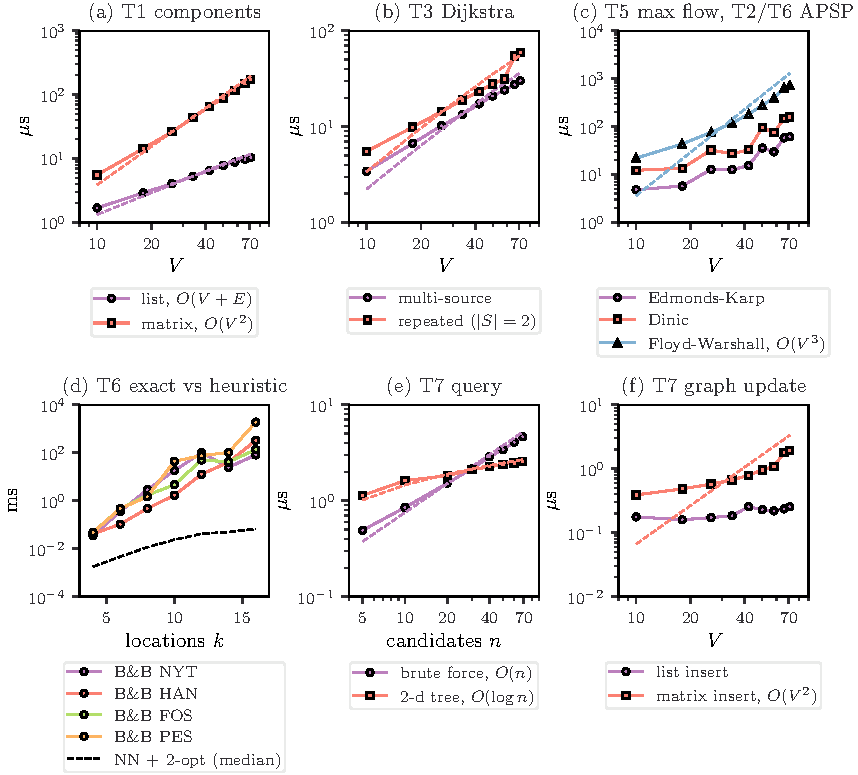
\includegraphics[width=\textwidth]{performance.pdf}
    \caption{Measured times (solid) against the theoretical cost model scaled to the data (dashed). All axes are logarithmic except the $k$ axis of (d), so that exponential growth in (d) appears as a straight line.}
    \label{fig:performance}
\end{figure}

\begin{table}[H]
\centering\footnotesize
\setlength{\tabcolsep}{4pt}
\caption{Median times in microseconds on the four instances; each column header gives the instance with $(V, E)$. Flow times cover both sectors; NN + 2-opt covers the full route; nearest-node times are for one query.}\label{tab:performance}
\begin{tabular}{lrrrr}
\toprule
\tablebody{performance}
\bottomrule
\end{tabular}
\end{table}

\subsection{Agreement with theory}
Most measurements follow their models. Component search grows with log-log slope about 0.9 on the adjacency list and 1.8 on the matrix (models 1 and 2), and the matrix is about 17 times slower at $V=71$, as $O(V^2)$ against $O(V+E)$ predicts for sparse graphs. Both Dijkstra variants follow $(V+E)\log V$, with slopes about 1.1 and 1.2. Repeated Dijkstra performs exactly twice the relaxations of the multi-source version and takes 1.4 times as long on the median subset and 2.0 times on the full PES network, where fixed overheads matter least.

Three measurements deviate from their models, each for an identifiable reason. The Floyd-Warshall time grows with slope about 1.8 instead of 3, because each of its $V$ steps is one vectorised NumPy update whose fixed cost dominates while the matrix has at most 5,041 cells; it still performs exactly $V^3$ elementary updates, and its curve steepens towards the $V^3$ reference as $V$ grows. Edmonds-Karp and Dinic grow far more slowly than $O(VE^2)$ and $O(V^2E)$ (Figure~\ref{fig:performance}c), because every source-sink pair needs at most four augmenting paths, each found by one $O(E)$ BFS; at this scale Edmonds-Karp is faster, about 2.5 times on the median sub-network and 1.6 to 2.2 times on the full instances, since Dinic's level graph and recursive blocking-flow search only pay off when a phase contains many augmenting paths. The matrix insertion grows about 5 times from $V=10$ to 71, much less than $V^2$, because copying a few thousand cells is cheap next to NumPy's allocation cost; the quadratic growth would dominate on larger networks.

Branch and bound is the only exponential cost. Its time multiplies by about 1.4 (NYT) to 2.2 (HAN) per added location, reaching about 2\,s at $k=16$ on PES, while NN + 2-opt stays below 0.1\,ms. The 2-d tree query grows logarithmically (3.5 to 11 distance evaluations) and beats brute force from about 30 candidates, but its build pays for itself only after a few tens of queries, so for the two or three insertions per instance brute force is sufficient.

\section{Results}\label{sec:results}

\paragraph{T1: representation.} Every instance is one connected component, so every junction can be supplied by some source. BFS on the matrix is 8.3 (NYT) to 22.6 (PES) times slower than on the list, because each visited vertex scans a full row. Memory is close at this size: a list entry is a Python tuple plus a float (about 120 bytes per pipe end) against 8 bytes per matrix cell, so the list is slightly larger on NYT (5.7 against 4.7 KiB), but the matrix grows quadratically and doubles the list on PES (44.6 against 23.3 KiB). The matrix only wins the pipe-existence query (67 against about 135 ns), so the list is the working representation and the matrix is used only for all-pairs tables.

\paragraph{T2: pipe lengths.} Table~\ref{tab:lengths} gives the length statistics. Length and capacity are distinct attributes (correlation $-0.65$ to $+0.13$). The FOS mesh keeps every pair within 1.75 times its straight-line distance, while NYT and HAN reach 4.73 and 3.32. PES is extreme: nodes 19 and 39 are 147 units apart but 4,146 by pipe, because PES is two dense clusters joined by few pipes. On average network distances are 19\% (FOS) to 83\% (PES) longer than straight lines, which is why T3 and T4 use $d_G$. The hash index answers a length query in 0.09\,\textmu s against 6.5\,\textmu s for a scan, and the sorted array finds the 9 PES pipes longer than 1,000 with 7 comparisons instead of 98.

\begin{table}[H]
\centering\small
\caption{Pipe lengths (coordinate units) and circuity $d_G/\lVert p_u-p_v\rVert$ over all node pairs.}\label{tab:lengths}
\begin{tabular}{lrrlrlrrrr}
\toprule
\tablebody{lengths}
\bottomrule
\end{tabular}
\end{table}

\paragraph{T3: sectors.} Figure~\ref{fig:freshness} shows the sectors (sizes in Table~\ref{tab:chain}). The pipes to close are 2--3, 11--9 and 20--16 in NYT; 7--8 and 14--15 in HAN; 18--19 and 19--20 in PES; and eight in the FOS mesh: 3--4, 28--9, 11--19, 27--16, 11--26, 16--29, 26--27 and 28--29. HAN's sectors are the most unequal (7 against 25 nodes) because source 13 sits behind a single 1,683-unit pipe at the network's edge. Multi-source Dijkstra used exactly half the heap operations of the repeated version (76 against 155 pops on PES).

\begin{figure}[H]
    \centering
    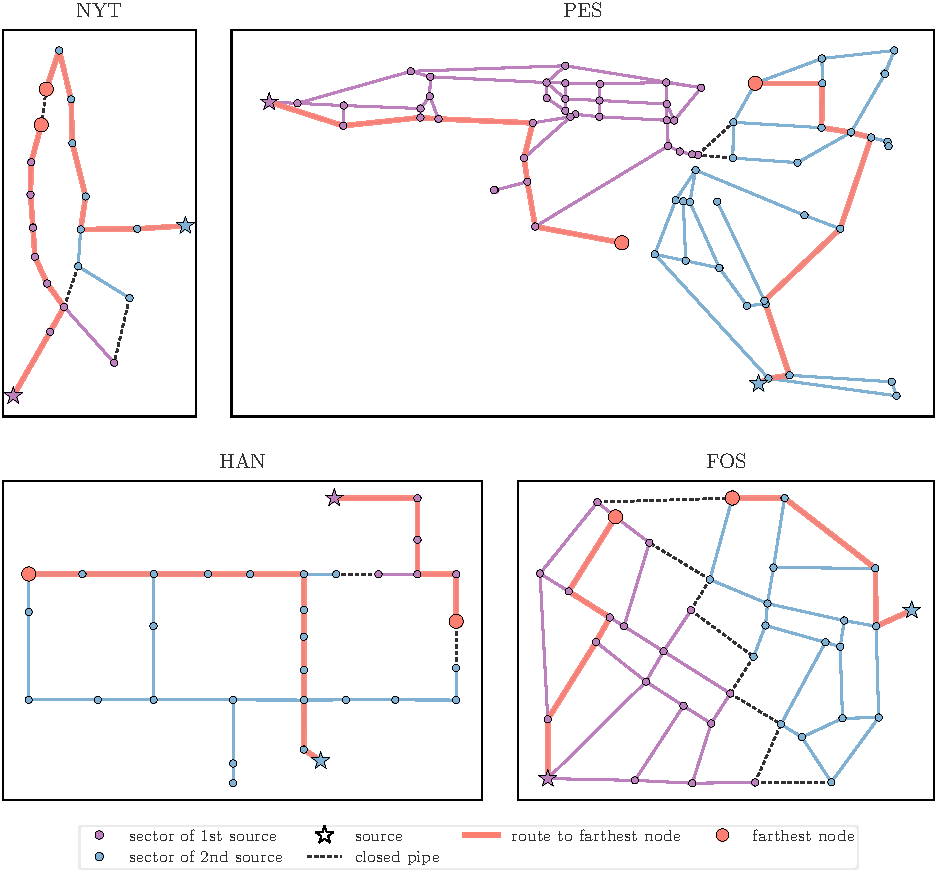
\includegraphics[width=0.92\textwidth]{freshness.pdf}
    \caption{T3 and T4. Sectors from multi-source Dijkstra (colour), closed pipes (dashed) and the shortest route from each source to the node of its sector that receives the oldest water.}
    \label{fig:freshness}
\end{figure}

\paragraph{T4: freshness.} Table~\ref{tab:chain} gives each sector's farthest node and distance; routes are drawn in Figure~\ref{fig:freshness} and listed in \texttt{04\_freshness}. Four of the eight (NYT 3 and 2, HAN 8, FOS 3) sit at a closed pipe, where the two supply areas meet; the others lie at the far end of their sector. Column ``Before'' divides the source's farthest distance in the open network by $d_G(s,t_s)$: sectorization reduces the worst water age a source is responsible for by 1.49 to 2.25 times in FOS and PES and by 2.75 times for HAN source 13; HAN source 1 is unaffected. Per node nothing changes, since closing $C$ leaves every distance to the node's own source intact.

\begin{table}[H]
\centering\small
\caption{Results chained per sector: size (T3), farthest node and distance (T4), maximum flow, capacity of the T4 route alone and minimum cut (T5).}\label{tab:chain}
\begin{tabular}{lrrrrrrrp{3.3cm}}
\toprule
\tablebody{chain}
\bottomrule
\end{tabular}
\end{table}

\paragraph{T5: maximum flow.} In six of the eight sectors the minimum cut is the single pipe at a leaf source (NYT, HAN, PES source 7) or leaf sink (PES 10), so the rest of the sector does not affect throughput. Comparing with the T4 route shows the difference between the two problems: PES source 1's shortest route carries only 101, but a second route into node 11 lets 151 reach node 10, and in the FOS mesh three disjoint bottleneck pipes carry 55 against 19 on the shortest route, and 58.8 against 17 in the other sector (Figure~\ref{fig:flows}). Making the cut pipes unlimited shows how capacity constrains the flow: the gain is nil in HAN, where every route is a chain of 16-capacity pipes, and reaches 3.6 times for FOS source 37 (58.8 to 211). Edmonds-Karp and Dinic always agree, with at most 4 augmenting paths.

\begin{figure}[H]
    \centering
    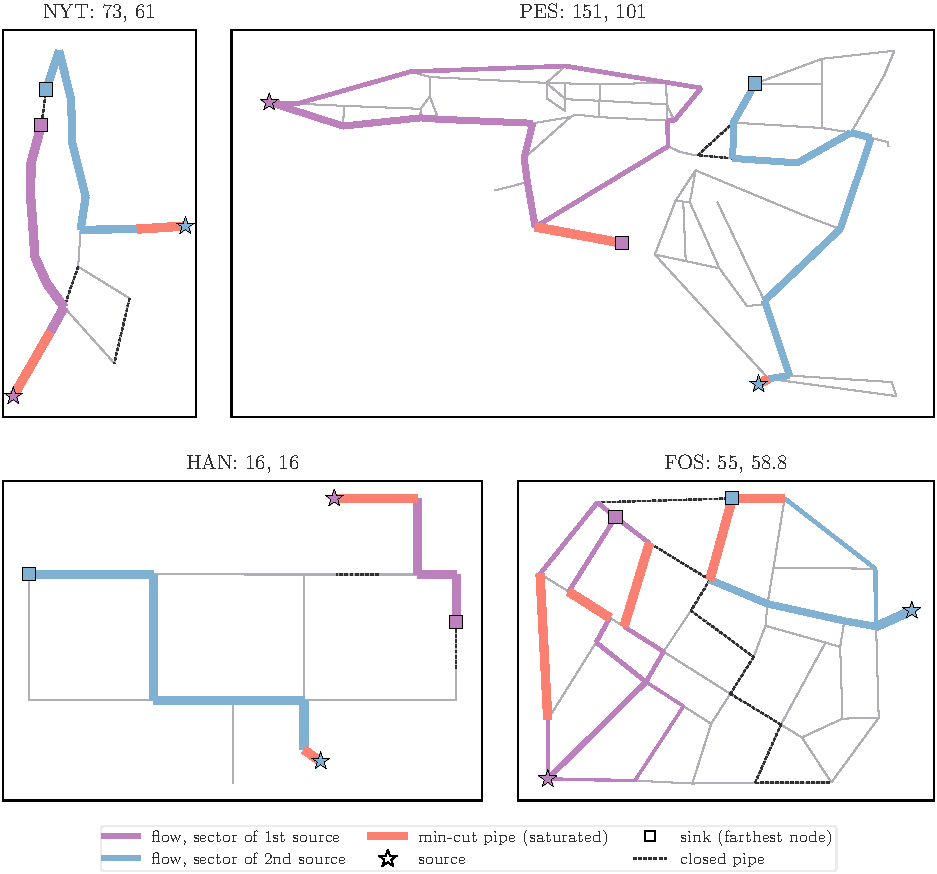
\includegraphics[width=\textwidth]{flows.pdf}
    \caption{T5 on the two meshed instances. Pipe width is proportional to flow; saturated minimum-cut pipes are highlighted. Titles give each sector's maximum flow.}
    \label{fig:flows}
\end{figure}

\paragraph{T6: sampling routes.} Table~\ref{tab:routes} compares the methods. NYT is solved exactly: the optimal walk has length 7,072 over 24 pipe traversals and walks both source branches there and back (Figure~\ref{fig:routes}a). For HAN, FOS and PES branch and bound does not finish within 60\,s, so their routes are 2-opt local optima, approximate and not certified: the MST bound is weak, especially on the near-tree HAN, where a walk traverses most pipes twice but the MST counts them once. On office-nearest subsets of $k=4,6,\dots$ nodes, solved exactly up to $k=18$ to 24, nearest neighbour is on average 15.9\% above the optimum (worst 37.8\%) and 2-opt 1.8\% (worst 15.8\%), optimal in 31 of 39 subsets (Figure~\ref{fig:routes}c).

\begin{table}[H]
\centering\small
\caption{Sampling routes. 2-opt gap: relative to the optimum when proven, otherwise an upper bound relative to the root lower bound. Walk pipes: pipe traversals of the expanded route.}\label{tab:routes}
\begin{tabular}{lrrrrlrrr}
\toprule
\tablebody{routes}
\bottomrule
\end{tabular}
\end{table}

\begin{figure}[H]
    \centering
    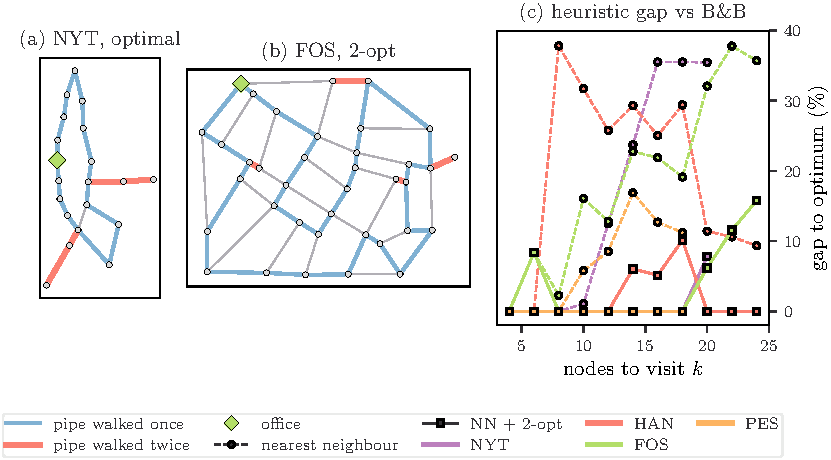
\includegraphics[width=\textwidth]{routes.pdf}
    \caption{T6. (a) Optimal NYT walk (7,072) and (b) best FOS walk found (30,424) from the office; pipes walked twice are highlighted. (c) Gap of nearest neighbour (dashed) and NN + 2-opt (solid) to the branch-and-bound optimum on office-nearest subsets.}
    \label{fig:routes}
\end{figure}

\paragraph{T7: expansion.} Table~\ref{tab:expansion} lists the insertions (Figure~\ref{fig:expansion}). The FOS point $(7071,9055)$ becomes node 38 linked to node 17, the connection drawn in the challenge slides. No new node is closest to an earlier new node, so insertion order does not matter here. On 2,000 random queries the 2-d tree evaluated on average 6.7 of 18 candidates on NYT and 11.0 of 69 on PES. Each insertion writes three list entries, whereas the matrix copies the whole table (10,225 cells for the two PES insertions).

\begin{table}[H]
\centering\small
\caption{New nodes, their nearest non-source node and the distance evaluations of each search.}\label{tab:expansion}
\setlength{\tabcolsep}{4pt}
\begin{tabular}{lrlrrrrr}
\toprule
\tablebody{expansion}
\bottomrule
\end{tabular}
\end{table}

\begin{figure}[H]
    \centering
    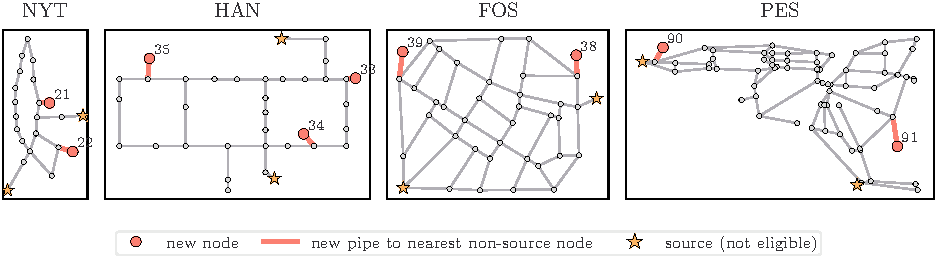
\includegraphics[width=\textwidth]{expansion.pdf}
    \caption{T7. Expanded networks: each new node is linked to its nearest non-source node.}
    \label{fig:expansion}
\end{figure}

\section{Conclusions}\label{sec:conclusions}
\paragraph{How the tasks relate.} The tasks form a chain. T2's lengths are the weights of every shortest path; T3 turns them into sectors; T4 reads the oldest-water node of each sector from the same Dijkstra tree; T5 uses that node as the sink of a flow problem restricted to the sector. T6 reuses T2's all-pairs distances as its metric closure, and T1 decides the representation all of them run on. The results also explain each other. The leaf sources found in the data stage are both the single-pipe bottlenecks of T5 and the dead ends the T6 walk must traverse twice. PES's extreme circuity in T2 reflects two clusters joined by few pipes, which is why separating its sectors needs only two closures in T3. T4 and T5 on the same source--sink pairs show concretely that the shortest route and the maximum flow are different problems: the route minimises length, the flow is set by the narrowest cut, and in the meshed FOS the flow is about three times what the shortest route alone could carry.

\paragraph{Cost and difficulty.} T6 is the only hard problem. Its exact solution grows exponentially with the number of locations, so optimality was proven only for NYT and for subsets of at most 24 nodes; for HAN, FOS and PES the routes are heuristic. Among the polynomial steps, Floyd-Warshall ($O(V^3)$) is the most expensive, and the adjacency matrix in general costs $O(V^2)$ where the list costs $O(V+E)$. Dijkstra, the flow algorithms and the nearest-node search are all fast at this scale; the flow algorithms run far below their worst-case bounds because the sectors need at most four augmenting paths. The cheap heuristics carry most of the value of the expensive method: 2-opt was within 1.8\% of the optimum on average. A selection hyper-heuristic over the same kind of moves made the heuristic routes more reliable across runs and shortened the best PES route by 2.3\%, still without a guarantee.

\paragraph{Limitations.} The model is purely graph-theoretic: there is no hydraulics (pressure, head loss, demand), capacities are taken as given numbers without units, and water age is taken as proportional to distance rather than to travel time. Flow is analysed for one source--sink pair per sector inside the closed sector, not for the whole network. Several conventions were needed and are stated where used: the treatment of PES's repeated pipe, the rejection of NYT's outlying new point, the sequential insertion of new nodes, and tie-breaking towards the earlier source (no ties occurred). The branch-and-bound bound is simple and weak on near-tree networks, so the full HAN, FOS and PES routes remain uncertified. Finally, the instances are small ($V\le71$), so performance conclusions rest on growth across subsets and are affected by Python interpreter overhead.


\pagebreak

\addcontentsline{toc}{section}{References}
\bibliographystyle{apalike}
\bibliography{references}

\clearpage
\begin{appendices}
\section{Sampling walks}\label{app:walks}
Table~\ref{tab:walks} lists the T6 walks of Table~\ref{tab:routes}, expanded from the tour of the metric closure into consecutive pipes. Each starts and ends at the office and visits every node; repeated nodes are where the walk passes through a junction again.

\begin{table}[H]
\centering\small
\caption{T6 closed walks from the office, as node sequences (optimal for NYT, NN + 2-opt for the others).}\label{tab:walks}
\begin{tabular}{lrp{12.2cm}}
\toprule
\tablebody{walks}
\bottomrule
\end{tabular}
\end{table}
\end{appendices}


\end{document}